\def\year{2015}
\documentclass[letterpaper]{article}
\usepackage{aaai}
\usepackage{fixbib}
\usepackage{times}
\usepackage{helvet}
\usepackage{courier}
%\usepackage[dvipdfmx]{graphicx}
\usepackage{graphicx}
\usepackage{amsmath}
\usepackage{amsfonts}
\usepackage{url}
\frenchspacing
\setlength{\pdfpagewidth}{8.5in}
\setlength{\pdfpageheight}{11in}
\pdfinfo{
/Title (Insert Your Title Here)
/Author (Put All Your Authors Here, Separated by Commas)}
\begin{document}
%
\title{Bayesian Optimization for Crowd Density Prediction}
\author{CS4246 Project: Planning and Decision Making in the Real World  \\ \\
{\bf Team 04} \\
Huang Wei Ling, A0101200R\\
Nathan Azaria, A0113011L\\
Ng Hui Xian Lynnette, A0119646X\\
Nguyen Duc Thien, A0093587M\\
Oh Shunhao, A0065475X\\
}
\maketitle
\begin{abstract}
Crowd density prediction is relevant to tackle issues in events such as resource management. Event space is usually limited and there are many concurrent activities at any point of time. Therefore, crowd density prediction is useful for the event committee to plan the layout and schedule of the programs in an event effectively and allows participants of the event to move around the event space efficiently so that they can benefit most out of the event. \\

In this report, we illustrate the use of Bayesian Optimization to find a set of reference points in an area. For each data point, we compute the shortest path distance from the data point to each of the reference points and used the outputs of the shortest path for GP regression to predict the crowd densities.
\end{abstract}

\section{Introduction}
In this report, we propose the use of Bayesian Optimization for crowd density prediction. Particularly, we discuss how Bayesian Optimization is used to find a set of reference points in an area for crowd density prediction, how we conduct training on the set of reference points chosen to find the optimal set of reference points that minimises the function $f(x)$ as well as the important requirements of our proposed application. \\

We will touch on the technical details which includes how we compute the shortest path, modelling the distance using GP regression, density and error computations. We will also outline the experimental plan we used to perform and evaluate the performance of Bayesian Optimization for crowd density prediction. \\

The rationale behind using Bayesian Optimization for crowd density prediction is to minimise the error by predicting whether a set of reference points given an environment setup is suitable to predict the crowd density in the environment.

\section{Crowd Density Prediction}

Bayesian Optimisation method is used to predict the crowd density by using a set of $3$ reference points from a known environment. In this section we describe the details of the use of Bayesian Optimization, to later present details on the specific algorithm for calculating the shortest paths and the use of GP regression in the implementation of the function $f(x)$ in Bayesian Optimization.

\subsection{Training of data}

For our proposed application, we are using a subset of the population in the area, $M$, which are the locations of people, to train the set of reference points selected. First, we divide $M$ into smaller groups. Each group is used together with the set of reference points to compute the shortest path distances and modelled using GP regression to predict the crowd density of $M$. Then, we can compute the error of the prediction with the set of $M$ locations of people and output this result to the Bayesian Optimization process to generate a new set of reference points which are more optimal than the previous set for training.

\subsection{Bayesian Optimization}

In general, the main objective of Bayesian Optimization is to find the optimal (maximum or minimum) of an unknown and costly $x$ to evaluate function $f$, which is to find $x^* = \text{argmax}_x f(x)$ or $x^* = \text{argmin}_x f(x)$. \\

In our proposed application of crowd density prediction, we are interested to minimise the function $f(x)$, which $f(x)$ refers to the error of the crowd density prediction. The $x$ in the function $f(x)$ refers to the input points $c_1, c_2, c_3$ which each of the input points is represented by the $x$ and $y$ coordinates of a location in the floor plan provided.  \\

Initially, we will pick 3 random input points of the locations of the floor plan to form $c_1, c_2, c_3$, and use these points together with the M as the inputs for the training of data. The output of the training of data will be the error of the crowd density prediction, $f(x)$, and $f(x)$ will be the input to the Bayesian Optimization process to optimise $x$, which is another set of input points $c_1, c_2, c_3$, for the next round of training of data. \\

The Bayesian Optimization is done with GPyOpt library, which is run with the Lower Confidence Bound acquisition function, as we seek to reduce the RMSE. We use a maximum iterations, or exploration horizon of 15;.The method used to optimize the acquisition function is fast\_random, which means the function runs only one optimizer in the best location. The input function $f$ that we optimize is the entire system of predicting the crowd density.

\subsection{Important Requirements}

An important requirement of our task is we must have the floor plan in order to perform Bayesian Optimisation for shortest path prediction. Our experiment uses 2 different floor plans from the same event which we apply Bayesian Optimization to each floor.\\

As we use time-series data for the Gaussian Process, there are potentially a large amount of data points, especially for time periods that last multiple days. Also, as our bayesian optimisation process optimises a function that includes running a Gaussian Process as part of its computation, thus the efficiency of the algorithm is very important, to allows the bayesian optimisation algorithm more time to do more iterations.\\

As we construct separate Gaussian Distributions for each person we can train the different gaussian processes in parallel, and so to speed things up, the computations can be distributed over multiple machines.


\section{Technical Approach}
The experiment is conducted using Python. For the Gaussian Process modelling and regression, we use the library Sheffield GPy with the help of Scipy and Numpy for numerical calculation and representation. The Bayesian Optimization process was done with the Sheffield GPyOpt library, an extension of the Gpy library. We use the data structure and data analysis tools provided by the module Pandas to store, access and analyze our dataset.

\subsection{Generating Shortest Path Coordinates}

We note that in the original data, the positions of each individual at any point of time is given in Cartesian coordinates $(x,y)$. The first step is thus to convert the existing Cartesian coordinates of each person's location specified in the data into a 3-tuple of shortest-path coordinates, $s_1, s_2, s_3$, referring to the shortest paths from the current position to each of the three reference points respectively.\\

\begin{figure}[!h]
  \centering
    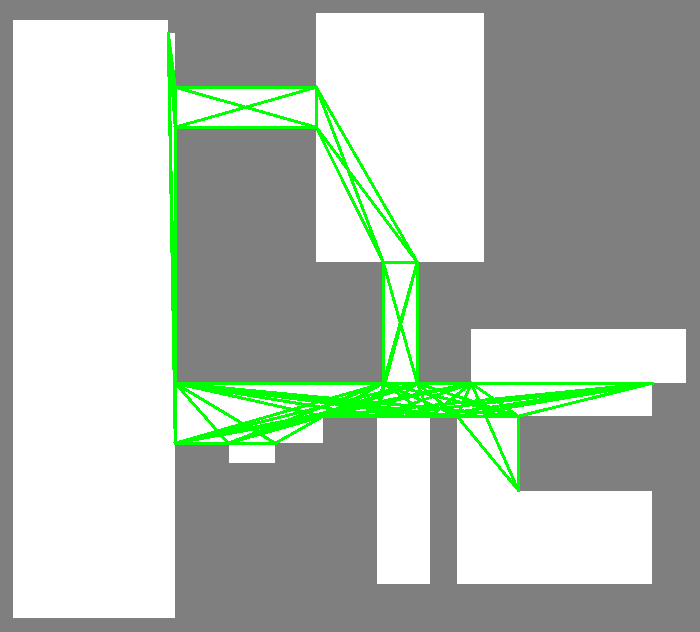
\includegraphics[width=170px]{diagrams/floor18visibilitygraph.png}
  \caption{Visibility Graph generated over the 18th floor of the Hotel Pennsylvania, New York City, building}
  \label{fig:floor18vg}
\end{figure}

Shortest path coordinates are computed using Any-Angle Pathfinding algorithms on grids. A floorplan of the area is used, and abstracted into a grid of blocked and unblocked tiles, representing impassable and passable areas in the actual space respectively. Then, for each $(x,y)$ coordinate in the data, we map it to the nearest unblocked tile on the grid. This can be done efficiently using Kd-trees.\\

\begin{figure}[!h]
  \centering
    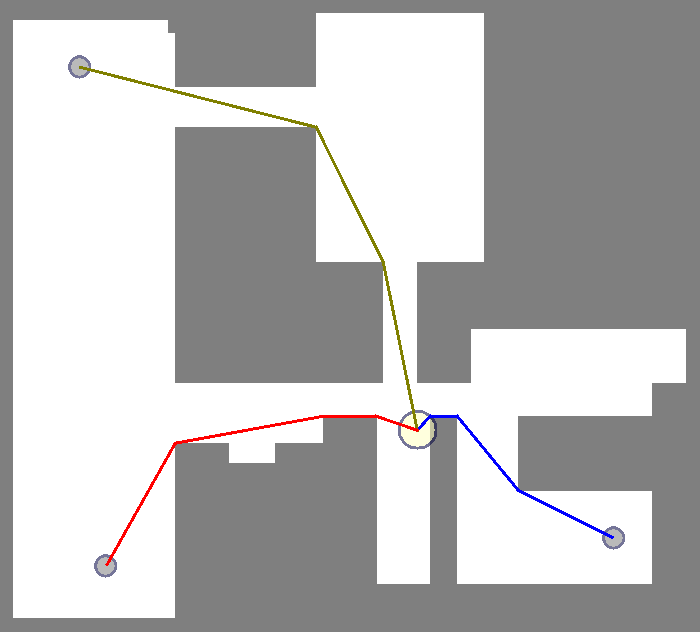
\includegraphics[width=170px]{diagrams/floor18shortestpaths.png}
  \caption{Shortest any-angle paths computed from a single point to three different reference points.}
  \label{fig:floor18sps}
\end{figure}

We then apply an optimal any-angle pathfinding algorithm to compute the shortest path from the $(x,y)$ coordinate to each of the three reference points. This generates three shortest-path queries for each user position. This shortest path computation can be done efficiently as a batch, on an approximately 100x100 grid by preprocessing a visibility graph like shown on Figure \ref{fig:floor18vg}, which can be reused to process each of the shortest path queries (Figure \ref{fig:floor18sps}). Running the A* algorithm on visibility graphs is an optimal offline algorithm for Any-Angle Pathfinding.\footnote{Visibility graph algorithm \url{https://github.com/Ohohcakester/Any-Angle-Pathfinding}}\\

Thus for each point, as there are three reference points, we obtain three shortest-path coordinates, $s_1, s_2, s_3$.

\subsection{Gaussian Processes for Probability Distributions}

In our GP model, each individual is modelled with a separate Gaussian Process. For each person in the data, the shortest-path coordinates, $s_1, s_2, s_3$ of the person is given at various points of time. As we seek to model the locations of each person as a function on time, the input location space (dependent variable) for our data is the time interval in which the data resides, and the target variable is a tuple $(s_1, s_2, s_3)$ in $\mathbb{R}^3$. \\

The hope is that with a good selection of reference points, the coordinates $s_1, s_2, s_3$ can be regarded as independent of each other without a significant loss of accuracy. From the regression, we obtain, at each point of time, a probability distribution of each of the coordinates $s_1, s_2, s_3$, described as a trivariate normal distribution $\mathcal{N}\tilde (\boldsymbol{\mu},\boldsymbol{\Sigma})$. \\

Several types of GP models were experimented with, including Stochastic Variance Gaussian Processes and Sparse Gaussian Processes. We also performed experiments with all the different types of kernels provided by the Sheffield GPy library, including linear kernel and white kernel. We also tweaked the input parameters, such as the variance of the kernels to experiment with the data. The GP model-variant that we proposed has the co-variance matrix and mean that fits the data the best. Figures \ref{fig:path1} and \ref{fig:path2} show the shortest paths to points 1 and 2 against time for User 3857 given the points in the first iteration. \\

Some of the kernels such as RBF kernel return matrices that are not positive semi-definite, hence causing an error in the next iteration of the GP regression. We hence use a squared exponential kernel with a variance of 1. We also add some noise to the kernel to simulate the noise variable in the GP model.

\begin{figure}[!h]
  \centering
    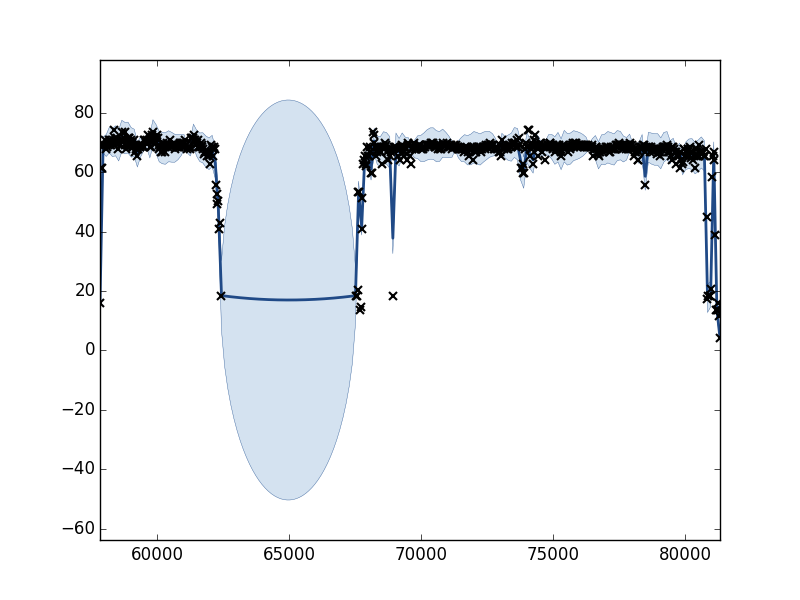
\includegraphics[width=200px]{diagrams/3587-path1.png}
  \caption{GP Regression for User 3587 of Shortest Paths to Point 1 against Time}
  \label{fig:path1}
\end{figure}

\begin{figure}[!h]
  \centering
    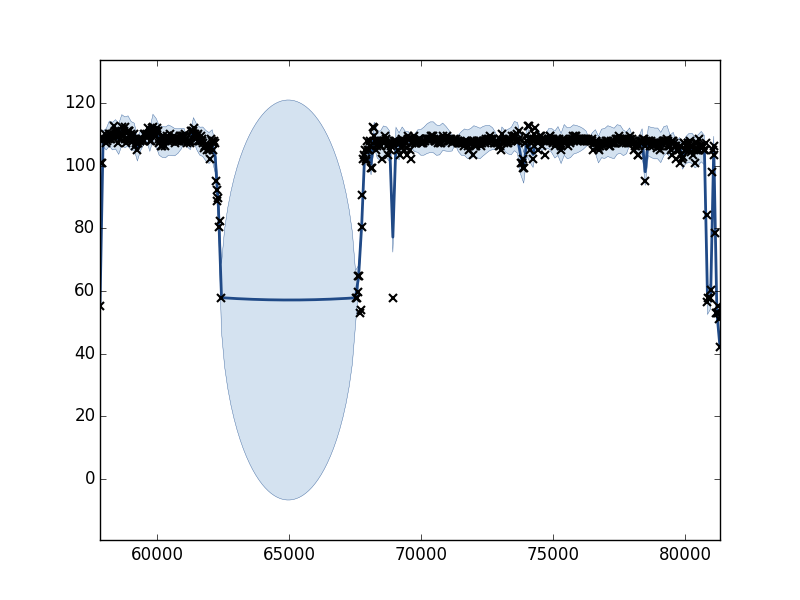
\includegraphics[width=200px]{diagrams/3587-path2.png}
  \caption{GP Regression for User 3587 of Shortest Paths to Point 2 against Time}
  \label{fig:path2}
\end{figure}

\subsection{Crowd Density Computation}

The use of shortest-path coordinates over Cartesian coordinates makes density computation more challenging. One can no longer simply select an arbitrary region (e.g. a rectangle) and integrate the probability distribution over all $x$ and $y$ values that fall within the region. One cannot even assume a one-to-one mapping between the shortest-path coordinates and the Cartesian coordinates. \\

Thus the integration has to be carried out differently. Instead of picking a rectangle in the Cartesian plane, we integrate over rectangles defined over the shortest-path coordinates. A rectangle is defined as the set 
\[\{(s_1,s_2,s_3) : a_1\leq s_1\leq b_1, a_2\leq s_2\leq b_2, a_3\leq s_3\leq b_3\}\]
for some boundary values $a_1,b_1,a_2,b_2,a_3,b_3 \in \mathbb{R}$.\\

\begin{figure}[!h]
  \centering
    
\includegraphics[width=170px]{diagrams/sprectangles.png}
  \caption{Illustration of the rectangles defined by shortest path coordinates, where $k_1 = k_2 = k_3 = 5$. Each colour corresponds to a different rectangle.}
  \label{fig:sprectangles}
\end{figure}

To define the rectangles, we first note that for each shortest-path coordinate $s_i$, $i \in \{1,2,3\}$, $s_i$ lies within some bounded interval $[0,D_i]$, for some $D_i > 0$. We then divide this interval into $k_i$ intervals of equal length. Interval $j$, where $j \in \{0,1,\cdots,k_i-1\}$ would correspond to the interval $[\frac{j}{k_i}D_i, \frac{j+1}{k_i}D_i]$.\\

Thus we define $\prod_{i=1}^3 k_i$ rectangles, each corresponding to a selection of intervals. For example, the rectangle indexed by the tuple $(0,2,1)$ would refer to $[0,\frac{D_1}{k_1}]\times [\frac{2D_2}{k_2},\frac{3D_2}{k_2}]\times [\frac{D_3}{k_3},\frac{2D_3}{k_3}]$. An illustration of what the rectangles look like in the original map is shown in Figure \ref{fig:sprectangles}.\\

\begin{figure}[!h]
  \centering
    
\includegraphics[width=170px]{diagrams/spsinglerectangle.png}
  \caption{Illustration of the rectangles defined by shortest path coordinates, where $k_1 = k_2 = k_3 = 5$. Each colour corresponds to a different rectangle.}
  \label{fig:sprectangles}
\end{figure}


At any point of time, for each rectangle, by integrating the probability distributions for each individual over the rectangle, we are able to obtain a prediction for the number of people within the rectangle. To obtain the predicted crowd density within the rectangle, we divide this value by the area of the region defined by the rectangle in the map.\\

The area of this rectangle can be estimated by the number of grid points within the rectangle. Using the same grid created from the floor plan earlier, the shortest paths from each point of the grid to each of the three reference points is computed. This gives us the shortest path coordinates for each point on the grid, allowing us to classify which rectangle each grid point belongs to, thus allowing us to count the number of grid points in each rectangle. \\

Thus by mapping each point in the grid to the density of the region it belongs to, we are able to obtain the crowd density at every point on the grid.

\subsection{Error Computation}

Thus we have calculated a predicted density distribution of $10\%$ of users used in the training set. These density distribution is then scaled up by a factor of $10$ to find an estimate of the actual density distribution of the $100$ users in the conference over the grid points. To obtain the actual density distribution over the grid points, for each grid point in the map, we count the number of people (out of $100$) within a $5$-unit radius of the grid point, and divide this by the area of the 5-unit circle to obtain the actual crowd density at that point. The root mean square error is then computed from the differences between the actual density distribution and the predicted density distribution, which is returned to the Bayesian Optimisation process. \\

This root mean square error is the value to be minimized in the Bayesian Optimisation process, where the function picks the optimal 3 points to estimate the crowd density in the hotel.


\section{Experimental Evaluation}

\subsection{Real-World Dataset}

We test our approach using a Attendee Meta-Data (AMD) Hope RFID Dataset from which data is collected from 1224 hackers attending The Last HOPE Conference from 18-20 July 2008, located in Hotel Pennsylvania, New York City.\\

The data set details the location of the attendees through the use of RFID badges that uniquely identify and track them across the conference space over the course of the conference. A plot of one of the position data over time of one of the attendees is shown in Figure .\\

This dataset was used as it has some convenient properties which allow us to construct an experiment to test our model. Firstly, the position data is usually taken at regular intervals of about $30$ seconds apart. Secondly, the data provided is exhaustive (as each attendee to the conference is tagged). \\

This provides enough information to find the actual number of people in each region at any point of time, by simply counting the number of people within the region, within in a time window of $[t-15,t+15)$, where $t$ is the target point of time.

\subsection{Experimental Setup}


For our experiment, $50$ time points are picked to be used for the test. These time points are chosen randomly from the time interval of the data, while ensuring a minimum gap of $200$ seconds between any two time points, and that there are at least $300$ unique active tags near that time point. This is done to avoid testing on periods where no or few people are active, like during the night, as the event spans multiple days.\\

At each chosen time point $t$, we obtain an actual density distribution using the same method as before: for each grid point in the map, count how many of the 1000 people within a $5$-unit radius of the grid point, and divide it by the area of the 5-unit circle to obtain the actual crowd density at that point. We then compute the predicted density using the same process as used in the training. During the training, the $100$ conference users were divided in to a $10$-$90$ proportion. $10\%$ of the user data were used for predicting the crowd density as defined by the other $90\%$ of the data. For our experimental evaluation, we use the same $100$ users, but this time, we use all $100\%$ of the user data, to make a prediction for the crowd density at each point, of all the $1224$ hackers attending the conference. Figures \ref{fig:t1dist} to \ref{fig:t2dist} show the actual and predicted crowd density distributions for the 18\textsuperscript{th} floor at two different points of time.\\

Then, for each time point $t$, at each point $p$ in the grid, the error at point $p$ is the difference between the predicted density and the actual densities at point $p$. By finding the root mean square error over all the points in the grid, we are able to obtain an error measure at each of the given time points.\\

\begin{figure}[h!]
  \centering
    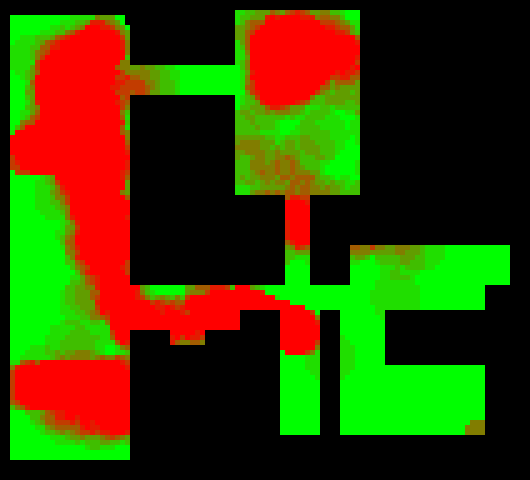
\includegraphics[width=170px]{diagrams/26-27_86-83_59-49_1216439889_actual.png}
  \caption{Actual density at $t=1216439889$ on the 18\textsuperscript{th} floor of the event.}
  \label{fig:t1dist}
\end{figure}

\begin{figure}[h!]
  \centering
    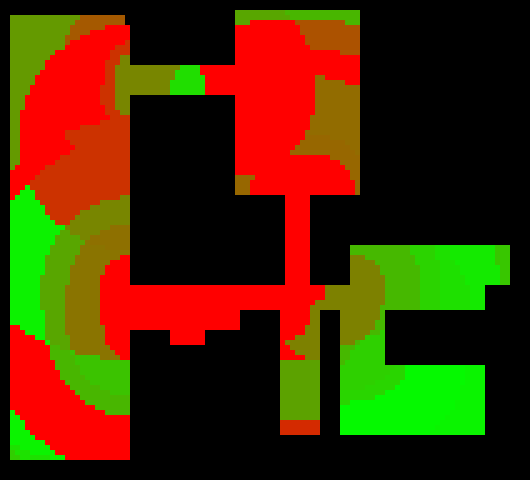
\includegraphics[width=170px]{diagrams/26-27_86-83_59-49_1216439889_predicted.png}
  \caption{Predicted density at $t=1216439889$ on the 18\textsuperscript{th} floor of the event.}
  \label{fig:t2dist}
\end{figure}

\begin{figure}[h!]
  \centering
    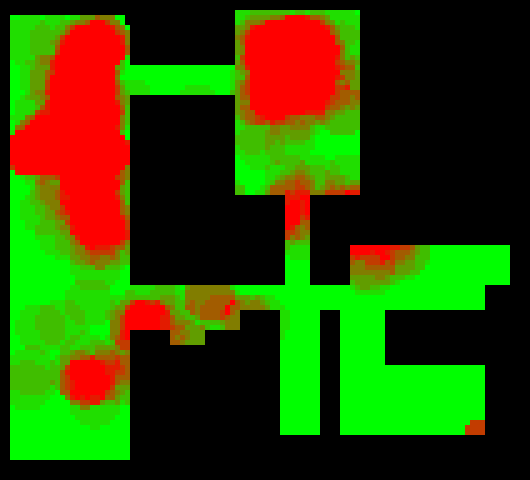
\includegraphics[width=170px]{diagrams/26-27_86-83_59-49_1216532755_actual.png}
  \caption{Actual density at $t=1216532755$ on the 18\textsuperscript{th} floor of the event.}
  \label{fig:t3dist}
\end{figure}

\begin{figure}[h!]
  \centering
    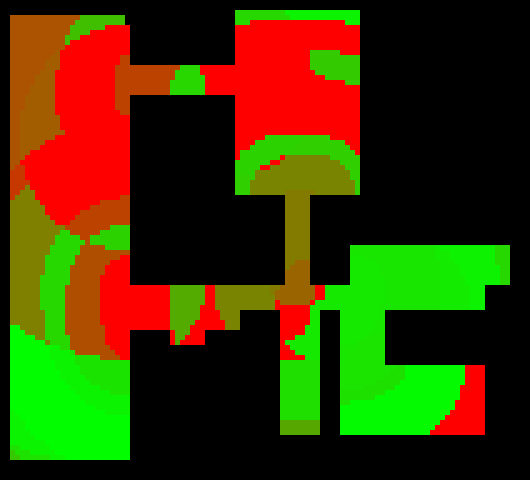
\includegraphics[width=170px]{diagrams/26-27_86-83_59-49_1216532755_predicted.png}
  \caption{Predicted density at $t=1216532755$ on the 18\textsuperscript{th} floor of the event.}
  \label{fig:t4dist}
\end{figure}

From the renders, we can see that the new distributions are much more expressive than those created by regressing gaussian distributions over the Cartesian $(x,y,z)$ coordinates. The shapes of the "dense" regions are able to wrap around objects, and are able to express crowds clustered at multiple locations, instead of having just one single peak value like shown in figure \ref{fig:xyzdist}.

\begin{figure}[h!]
  \centering
    
\includegraphics[width=170px]{diagrams/1_1216440525p.png}
  \caption{What the crowd density distribution looks like if we regressed over $x,y,z$ coordinates.}
  \label{fig:xyzdist}
\end{figure}


\subsection{Additional Insights}

We note that due to limitations of our pathfinding algorithms and lack of knowledge of how individuals travel between floors (though we strongly believe they use an elevator), we did the density prediction only over one floor. However, with sufficient knowledge and the correct pathfinding algorithms that allow navigation in three-dimensional spaces (e.g. using navigation meshes), we are able to model all the floors in an entire building with a single gaussian distribution. This will make much better path predictions, as currently, there are many gaps in the data arising from the individual not being in the current floor. Modelling an individual's movement over an entire building at once would create a more continuous path trajectory.\\

However, with the shortest paths coordinates, we lose the ability to integrate the gaussian processes over any arbitrary region to compute the crowd density within that area. The regions are instead defined by the boundaries of the rectangles, which are controlled by the positions of the reference points.\\

Thus, it is not easy to obtain a smooth crowd density distribution over the space without a large number of integrations over very small shortest-path coordinate rectangles.\\


\subsection{Improvement}


\section{Conclusion}

The goal of the current work is to optimimse the set of reference points that allows for predicting of crowd density. We described a framework for modeling shortest path distance using the GP model for density and error computations, we demonstrated that our approach is able to represent the dataset a lot more closely than regressing over $x,y,z$ coordinates. we have as well as predict the population density of a known environment.

\section{6. Main Roles of Each Member}
\begin{itemize}
\item \textbf{Wei Ling}: 
Writing of the report, keeping track of requirements, and research.
\item \textbf{Nathan}: 
Setting up of the experiment and running the tests using the dataset.
\item \textbf{Lynnette}: 
Setting up and experimenting with the various libraries and available tools, and fine-tuning the Gaussian Process models
\item \textbf{Thien}: 
Setting up and experimenting with the various libraries and available tools, and fine-tuning the Gaussian Process models
\item \textbf{Shunhao}: 
Problem formulation and modelling, mathematics, creating the visualisations and experiment, and writing the report.
\end{itemize}

\bibliographystyle{aaai}
\bibliography{report}

\end{document}
